\chapter{Java虚拟机}
课前思考:
\begin{itemize}
	\item Java语言如何实现跨平台?
	\item 什么是Java虚拟机(JVM)?
	\item JVM的内存是如何划分的?
	\item JVM的垃圾回收机制都有哪些?
\end{itemize}
\section{Java虚拟机概念}
\subsection{什么是Java虚拟机?}
\begin{itemize}
	\item Java虚拟机是一个想象中的机器,在实际的计算机上通过软件模拟来实现。
	Java虚拟机有自己想象的硬件,如处理器、堆栈、寄存器、还有相应的指令系统。
\end{itemize}
\begin{figure}[!h]
	\centering
	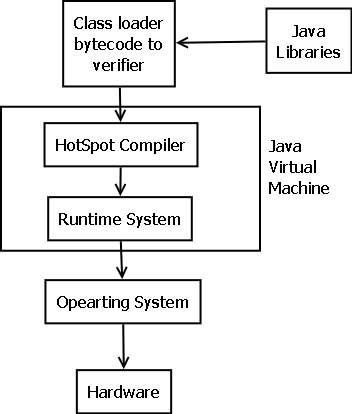
\includegraphics[width=0.5\textwidth]{image/JVM.png}
	\caption{Java运行环境}
\end{figure}
\subsection{为什么使用JVM?}
\begin{itemize}
	\item 实现Java的跨平台特性
	\item 把目标代码编译成字节码
\end{itemize}
\par 分为四层:应用程序层、Java平台层、操作系统层、硬件层。
\subsection{Java虚拟机的生命周期}
\begin{enumerate}
	\item 一个运行中的Java虚拟机有着一个清晰的任务:执行Java任务。程序开始执行时它才运行,
	程序结束时它就停止。每个Java程序会单独运行一个Java虚拟机。
	\subitem 通过命令行启动JVM:java classname
	\item JVM总是开始于一个main()方法,这个方法必须是public,返回void。
	直接接受一个字符串数组。在程序执行时,必须给Java虚拟机指明这个包含有main()方法的类名。
	\subitem public static void main(String[] args){}
	\item main()方法是程序的起点,它被执行的线程初始化为程序的初试线程。程序中其他的线程都由它来启动。
	Java中线程分为两种:守护线程(daemon)和普通线程(non-daemon)。
	\subitem 守护线程是JVM自己使用的线程,比如负责垃圾收集的线程,也可以把自己的程序设置为
	守护线程,包含main()方法的初始线程不是守护线程。
	\item 只要JVM中还有普通线程在执行,JVM就不会停止,如果有足够的权限,就可以调用exit()终止程序。
\end{enumerate}
\subsection{JVM的体系结构}
在JVM的规范中定义了一系列的子系统、内存区域、数据类型和使用指南。
这些组件构成了JVM的内部结构,它们不仅仅为JVM的实现提供了清晰的内部结构,
更是严格规定了JVM实现的外部行为。
\par 每个JVM都有一个类加载子系统(class loader subsystem),负责加载程序中的类型(类class和接口interface),
并赋予唯一的名字。每一个JVM都有一个执行引擎(execution engine)负责执行被加载类中包含的指令。
\subsection{JVM中使用的数据类型}
\begin{itemize}
	\item 所有JVM中使用的数据都有确定的数据类型,数据类型和操作都在JVM规范中严格定义。
	Java中的数据类型分为原始数据类型(primitive types)和引用数据类型(reference type)。
	\item 在JVm中还存在一个Java语言中不能使用的原始数据类型--返回值类型(return value)。
	这种数据类型被用来实现Java中的“finally classes”。
	\item 引用类型可能被创建为:类类型(class type),接口类型(interface type),
	数组类型(array type)。它们都引用了被动态创建的对象。当引用类型引用null时,说明没有引用任何对象。
\end{itemize}

\section{Java虚拟机内存划分}
\subsection{JVM内存区域}
\begin{figure}[!h]
	\centering
	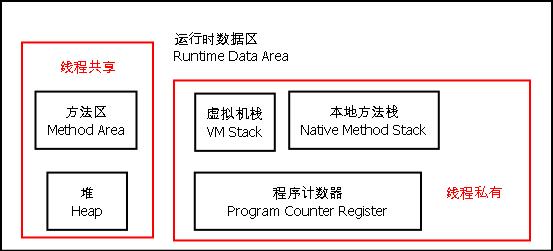
\includegraphics[width=0.7\textwidth]{image/JVM-Merory.png}
	\caption{JVM内存区域}
\end{figure}
\subsection{程序计数器}
\begin{itemize}
	\item JVM将这个计数看作当前执行某条字节码的行数,会根据计数器的值来选去需要执行的操作语句。
	这个属于线程私有,不可共享,如果共享会导致计数混乱,无法准确的执行当前线程需要执行的语句。
	\item 该区域不会出现任何OutOfMemoryError的情况。
\end{itemize}
\subsection{虚拟机栈}
\begin{itemize}
	\item 虚拟机栈就是指经常说到的栈内存。Java中每一个方法从调用直至执行完成的过程,就对应着一个栈帧在虚拟机栈中
	入栈到出栈的过程。
	\item 如果线程请求的栈深度大于虚拟机所允许的深度,将抛出StackOverflowError异常;
	如果虚拟机栈可以动态扩展(当前大部分的Java虚拟机都可动态扩展,只不过Java虚拟机规范中也允许固定长度的虚拟机栈),
	如果扩展时无法申请到足够的内存,就会抛出OutOfMemoryError异常。
\end{itemize}
\subsection{本地方法栈}
\begin{itemize}
	\item 本地方法栈用来执行本地方法,抛出异常的情况和虚拟机栈一样。而虚拟机栈用来执行Java方法。
\end{itemize}
\subsection{堆}
\begin{itemize}
	\item 是JVM中内存最大、线程共享的一块区域。唯一的目的是存储对象实例。这里也是垃圾收集器主要收集的区域。
	由于现代垃圾收集器采用的是分带手机算法,所以Java堆也分为新生代和老生代。
	\item 可以通过参数-Xmx(JVM最大可用内存)和-Xms(JVM初始内存)来调整堆内存,
	如果扩大至无法继续扩展时,会出现OutOfMemoryError的错误。
\end{itemize}
\subsection{方法区}
\begin{itemize}
	\item JVM中内存共享的一片区域,用来存储类信息、常量、静态变量、class文件。
	垃圾收集器也会对这部分区域进行回收,比如常量池的清理和类型的卸载。
	\item 方法区内存不够用的时候,也会抛出OutOfMemoryError错误。
\end{itemize}

\section{Java虚拟机类加载机制}
\subsection{虚拟机类加载机制的概念}
\noindent 1. 虚拟机把描述类的数据从class文件加载到内存,并对数据进行校验、
转换解析和初始化,最初形成可以被虚拟机直接使用的Java类型。
\\ 2. Java语言里,类型的加载和连接过程是在程序运行期间完成的。
\subsection{类的生命周期}
\begin{itemize}
	\item 加载loading
	\subitem 通过一个类的全限定名来获取此类的二进制字节码。
	\subitem 将这个字节码所代表的静态存储结构转化为方法区的运行时数据结构。
	\subitem 在Java堆中生成一个代表这个类的Class对象,作为方法区这些数据的访问入口。
	\item 验证verfication
	\subitem 虚拟机规范:验证输入的字节流是否符合Class文件的存储格式,否则抛出一个java.lang.VerifyError异常。
	\subitem 文件格式验证:验证字节流是否符合Classs文件格式的规范,并且能被当前版本的虚拟机处理。
	经过这个阶段的验证,字节流进入内存的方法区中进行存储。
	\subitem 元数据验证:对类的源数据信息进行语义校验,保证不存在不符合Java语言规范的元数据信息。
	\subitem 字节码验证:进行数据流和控制流分析,对类的方法体进行校验分析,
	保证被校验的类的方法在运行时不会做出危害虚拟机安全的行为。
	\subitem 符号引用验证:发生在虚拟机将符号引用转化为直接引用的时候(解析阶段),
	对常量池的各种符号引用的信息进行匹配性的校验。
	\item 准备preparation
	\subitem 准备阶段是正式为类变量分配内存并设置类变量初始值(各数据类型的零值)的阶段,这些内存将在方法区中进行匹配。
	但是如果类字段的字段属性表中存在ConstantValue属性,那在准备阶段变量值就会初始化为ConstantValue属性指定的值。
	\subitem public static final int value = 122;
	\item 解析resoulution
	\subitem 解析阶段是在虚拟机将常量池内的符号引用替换为直接引用的过程。
	\subitem 符号引用:符号引用以一组符号来描述所引用的目标,符号可以是任何形式的字面量,只要使用时能无歧义地定位到目标即可。
	符号引用与虚拟机实现的内存布局无关,引用的目标并不一定已经加载到内存中。
	\subitem 直接引用:直接引用是直接指向目标的指针、相对偏移量或者一个能间接定位到目标的句柄。
	如果有了直接引用,那引用的目标必定已经在内存中存在。
	\item 初始化initialization
	\subitem <clinit>()方法:由编译器自动收集类中所有类变量的赋值动作和静态语句块中
	语句合并并发生,收集的顺序是由语句在源文件中出现的顺序决定的。
	\subitem 该方法与实例构造器<init>()不同,不需要显示的调用父类构造器。
	\subitem <cinit>()方法对于类或接口来说不是必须的。
	\subitem 执行接口的<clinit>()不需要先执行父接口的<clinit>()方法。
	\subitem 虚拟机会保证一个类的<clinit>()方法在多线程环境中被正确的加锁和同步。
	\item 使用using
	\item 卸载unloading
\end{itemize}
\subsection{类的主动引用}
\begin{itemize}
	\item 遇到new、getstatic、putstatic、invokestatic这四个字条码指令时(使用new实例化对象的时候、读取或设置一个类的静态
	字段、调用一个类的静态方法)。
	\item 使用java.lang.reflet包的方法对类进行反射调用的时候。
	\item 当初始化一个类的时候,如果发现其父类没有进行过初始化,则需要先触发其父类的初始化。
	\item 当虚拟机启动时,虚拟机会初始化主类(包含main方法的那个类)。
\end{itemize}
\subsection{类的被动引用}
\begin{itemize}
	\item 通过子类引用父类的静态字段,不会导致子类初始化(对于静态字段,只有直接定义这个字段的类才会被初始化)。
	\item 通过数组定义类应用类:ClassA[] array = new ClassA[10]。触发了一个名为LClassA的
	类的初始化,它是一个由虚拟机自动生成的、直接继承与Object的类,创建动作由字节码指令newarray触发。
	\item 常量会在编译阶段存入调用类的常量池。
\end{itemize}
\section{判断对象是否存活算法及对象引用}
\subsection{什么是垃圾回收?}
当一个对象没有引用指向它时,这个对象就称为无用的内存(垃圾),就必须进行回收,以便用于
后续其他对象的内存分配。
\subsection{引用计数算法}
实现简单,判断效率高,在很大情况下,它都是一个不错算法,但是Java语言没有选用引用
计数算法管理内存,其中最主要的一个原因是它很难解决对象之间相互循环引用的问题。
\par ObjA.obj = ObjB;
\par ObjB.obj = ObjA
\subsection{可达性分析算法(根搜索算法)}
\begin{itemize}
	\item 在主流的商用程序语言中(Java),都是可达性分析判断对象是否存活的。
	\item 根搜索算法是从离散数学中的图论引入的,程序把所有的引用关系看一张图,从
	一个节点GC ROOT开始,如果一个节点与GC ROOT之间没有引用链的存在,该节点视为垃圾回收的对象。
\end{itemize}
\par 在Java中,作为GC Roots对象包括:
\begin{enumerate}
	\item 虚拟机栈(栈帧中的本地变量表)中引用的对象;
	\item 方法区中的类静态属性引用的对象;
	\item 方法区中的常量引用的对象;
	\item 本地方法栈中JNI的引用的对象。
\end{enumerate}
\textbf{对象引用-强引用}
\begin{itemize}
	\item 只要引用存在,垃圾回收器永远不会回收
	\subitem Object obj = new Object();
	\item obj对象对后面new Object有一个强引用,只有当obj这个引用被释放之后,
	对象才会被释放掉。
\end{itemize}
\textbf{对象引用-软引用}
\begin{itemize}
	\item 非必须引用,内存溢出之前进行回收,可以通过以下代码实现:
	\begin{lstlisting}[language=java]
Object obj = new Object();
SoftReference<Object> sf = new SoftReference<Obj>(obj);
obj = null;
sf.get();
	\end{lstlisting}
	\item 软引用主要用户实现类似缓存的功能,在内存足够的情况下直接通过软引用取值,
	无需从繁忙的真实来源查询数据,提升速度;当内存不足时,自动删除这部分
	缓存数据,从真正的来源查询这些数据。
\end{itemize}
\textbf{对象引用-弱引用}
\begin{itemize}
	\item 在第二次垃圾回收时,可以通过如下代码实现:
	\begin{lstlisting}[language=java]
Object obj = new Object();
WeakReference<Object> wf = new WeakReference<Object>(obj);
obj = null;
wf.get();
wf.isEnQueued();
	\end{lstlisting}
	\item 弱引用主要用于监控对象是否已经被垃圾回收器标记为即将回收的垃圾,
	可以通过弱引用的isEnqueued方法返回对象是否被垃圾回收器回收。
\end{itemize}
\textbf{虚引用(幽灵/幻影引用)}
\begin{itemize}
	\item 在垃圾回收时回收,无法通过引用取到对象值,可以通过如下代码实现:
	\begin{lstlisting}[language=java]
Object obj = new Object();
PhantomReference<Object> pf = new PhantomReference<Object>(obj);
obj = null;
pf.get();
pf.isEnQueued();
	\end{lstlisting}
	\item 主要用于检测对象是否已经从内存删除
\end{itemize}

\section{分代垃圾回收}
\subsection{分代垃圾回收的提出}
\begin{itemize}
	\item 在Java中,没有显示的提供分配内存和删除内存的方法。将引用对象设置为null
	或者调用System.gc()来释放内存。
	\item 在Java中,开发人员无法显示删除内存,所以垃圾收集器会发现不需要(垃圾)的对象,
	然后删除它们,释放内存。
	\item 基于以上两点,提出分代垃圾收集器。
	\subitem 1. 绝大数对象在短时间内变得不可达;
	\subitem 2. 只有少量年老对象引用年轻对象。
\end{itemize}
\subsection{年轻代和老年代}
\noindent \textbf{年轻代:}新创建的对象都存放在这里。因为大多数对象很快变得不可达,
所以大多数对象在年轻代中创建,然后消失。当对象从这块内存区域消失时,则成为发生了一次“minor GC”。
\\ \textbf{老年代:}没有变得不可达,存活下来的年轻代对象被复制到这里。这块内存
区域一般大于年轻代。因为它更大的规模,GC发生的次数比年轻代的少。
对象从老年代消失时,则称“major GC”(或“full GC”)发生了。
\subsection{年轻代组成部分}
\begin{itemize}
	\item 年轻代总共有3块空间:1块Eden区,2块Survivor区。各个空间的执行顺序如下:
	\subitem 绝大多数新创建的对象分配在Eden区;
	\subitem 在Eden区发生GC后,存活的对象移到其中一个Survivor区。
	\subitem 一旦一个Survivor已满,存活的对象移动到另外一个Survivor区。
	然后之前那个空间已满Survivor区将置为空,没有任何数据。
	\subitem 经过多次这样步骤依旧存活的对象将被移到老年代。
\end{itemize}
\section{典型的垃圾收集算法}
\subsection{Mark-Sweep(标记-清除))算法}
最基础的垃圾回收算法,因为它最容易实现,思想也是最简单的。标记-清除算法分为两个阶段:标记阶段和清除阶段。
标记阶段的任务是标记处所有需要被回收的对象,清除阶段就是回收被标记的对象所占用的空间。
\\ 缺点:容易产生碎片,碎片太多会导致后续过程中需要为大对象分配空间时无法找到足够的空间
而提前触发的一次垃圾手机动作。
\subsection{Copying(复制)算法}
为了解决Mark-Sweep算法的缺陷,Coping算法就被提出来。它将可用内存按容量划分为大小相等的两块,
每次只使用其中的一块。当这一块的内存使用完了,就将还存活着的对象复制到另外一块上面,然后再把
已使用的内存空间一次清理掉,这样一来就不容易出现内存碎片的问题。
\par 这种算法虽然实现简单,运行高效且不容易产生内存碎片,但是却对内存空间的使用
做出了高昂的代价,因为能够使用的内存缩减到原来的一半。
\par Copying算法的效率跟存活的对象的数目多少有很大关系,如果存活对象很多,那么Copying算法的效率将会大大降低。
\subsection{Mark-Compat(标记整理)算法}
为了解决Copying算法的缺陷,充分利用了内存空间,提出了Mark-Compact算法。
该算法标记阶段和Mark-Sweep一样,但是完成标记之后,它不是直接清理可回收对象,
而是将存活对象都向一端移动,然后清理掉边界外的内存。
\subsection{Generational Collection(分代收集)算法}
分代收集算法是目前大部分JVM的垃圾收集器采用的算法。它的核心思想是根据对象存活的生命周期
将内存划分为若干不同的区域。一般情况下将堆区划分为老年代(Tenured Feneration)和新生代
(Young Generation),老生代的特点是每次垃圾收集时只有少量对象需要被回收,而新生代的特点是
每次垃圾回收时都有大量的对象需要被回收,那么就可以根据不同代的特点采取最合适的收集算法。
\par 目前大部分垃圾收集器对于新生代都采取Copying算法,因为新生代中每次垃圾回收都要回收大部分对象,
也就是说需要复制的操作次数较少,但是实际中并不是按照1:1的比例来划分新生代的空间的,一般来说是将新生代划分为一块
较大的Eden空间和两块较小的Survivor空间,每次使用Eden空间和其中一块Survivor空间,当进行回收时,将Eden和Survivor中还存活的对象复制到另一块Survivor空间中,
然后清理掉Eden和刚才使用过的Survivor空间。
\par 对于老年代的特点是每次回收都只回收少量对象,一般使用的是Mark-Compact算法。
\par \textbf{注意:}在堆区之外还有一个代就是永久代(Permanent Generation),它用来存储class类、常量、
方法描述等。对永生代的回收主要回收两部分内容:废弃常量和无用的类。

\section{典型的垃圾收集器}
\subsection{Serial/Serial Old}
Serial/Serial Old收集器是最基本最古老的收集器,它是一个单线程收集器,
并且在它进行垃圾收集时,必须暂停所有用户线程。Serial收集器是针对新生代的收集器,采用的是
Copying算法,Serial Old收集器是针对老年代的收集器,采用的是Mark-Compact算法。它的优点是实现简单高效,
但是缺点是会给用户带来停顿。
\subsection{ParNew}
\begin{itemize}
	\item ParNew收集器是Serial收集器的多线程版本,使用多个线程进行垃圾收集。
\end{itemize}
\subsection{Parallel Scavenge}
\begin{itemize}
	\item Parallel Scavenge收集器是一个新生代的多线程收集器(并行收集器),
	它在回收期间不需要暂停其他用户线程,其使用的是Copying算法,该收集器与前两个收集器有所不同,
	它主要是为了达到一个可控的吞吐量。
	\item Parallel Old是Parallel Scavenge收集器的老年代版本(并行收集器),
	使用多线程和Mark-Compact算法。
\end{itemize}
\subsection{CMS}
CMS(Current Mark Sweep)收集器是一种以获取最短回收停顿时间为目标的收集器,
它是一种并发收集器,采用的是Mark-Sweep算法。
\subsection{G1}
\begin{itemize}
	\item G1收集器是当今收集器技术发展最前沿的成果,它是面向服务端应用的收集器,它能充分利用多CPU、
	多核环境。因此它是一款并行与并发收集器,并且它能建立可预测的停顿时间模型。
\end{itemize}